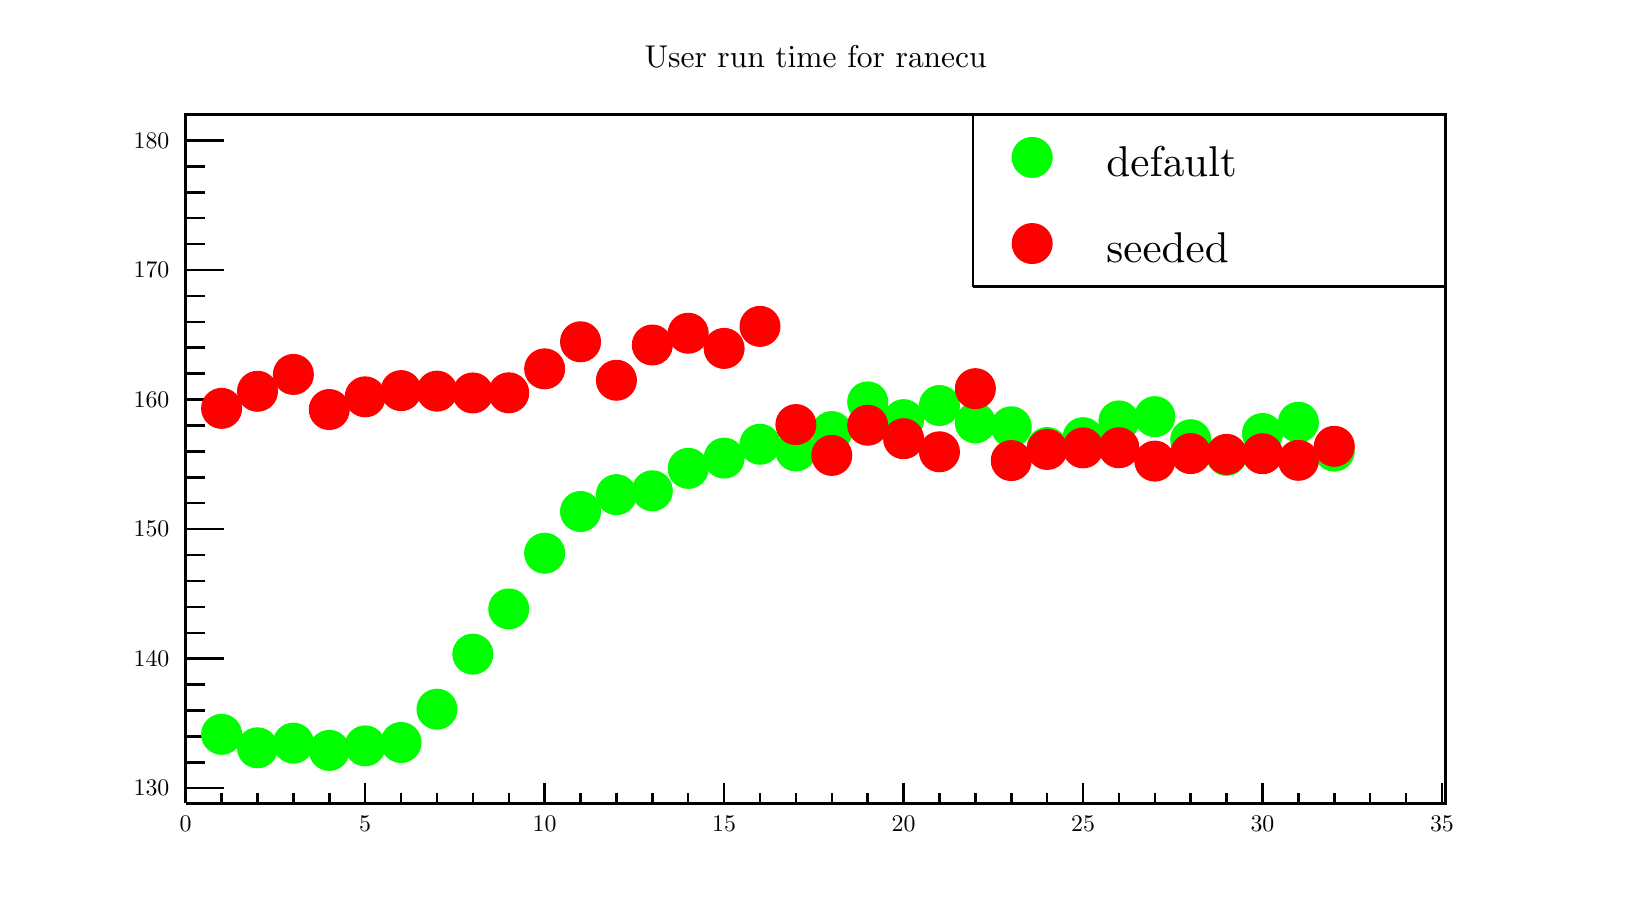
\begin{tikzpicture}
\pgfdeclareplotmark{cross} {
\pgfpathmoveto{\pgfpoint{-0.3\pgfplotmarksize}{\pgfplotmarksize}}
\pgfpathlineto{\pgfpoint{+0.3\pgfplotmarksize}{\pgfplotmarksize}}
\pgfpathlineto{\pgfpoint{+0.3\pgfplotmarksize}{0.3\pgfplotmarksize}}
\pgfpathlineto{\pgfpoint{+1\pgfplotmarksize}{0.3\pgfplotmarksize}}
\pgfpathlineto{\pgfpoint{+1\pgfplotmarksize}{-0.3\pgfplotmarksize}}
\pgfpathlineto{\pgfpoint{+0.3\pgfplotmarksize}{-0.3\pgfplotmarksize}}
\pgfpathlineto{\pgfpoint{+0.3\pgfplotmarksize}{-1.\pgfplotmarksize}}
\pgfpathlineto{\pgfpoint{-0.3\pgfplotmarksize}{-1.\pgfplotmarksize}}
\pgfpathlineto{\pgfpoint{-0.3\pgfplotmarksize}{-0.3\pgfplotmarksize}}
\pgfpathlineto{\pgfpoint{-1.\pgfplotmarksize}{-0.3\pgfplotmarksize}}
\pgfpathlineto{\pgfpoint{-1.\pgfplotmarksize}{0.3\pgfplotmarksize}}
\pgfpathlineto{\pgfpoint{-0.3\pgfplotmarksize}{0.3\pgfplotmarksize}}
\pgfpathclose
\pgfusepathqstroke
}
\pgfdeclareplotmark{cross*} {
\pgfpathmoveto{\pgfpoint{-0.3\pgfplotmarksize}{\pgfplotmarksize}}
\pgfpathlineto{\pgfpoint{+0.3\pgfplotmarksize}{\pgfplotmarksize}}
\pgfpathlineto{\pgfpoint{+0.3\pgfplotmarksize}{0.3\pgfplotmarksize}}
\pgfpathlineto{\pgfpoint{+1\pgfplotmarksize}{0.3\pgfplotmarksize}}
\pgfpathlineto{\pgfpoint{+1\pgfplotmarksize}{-0.3\pgfplotmarksize}}
\pgfpathlineto{\pgfpoint{+0.3\pgfplotmarksize}{-0.3\pgfplotmarksize}}
\pgfpathlineto{\pgfpoint{+0.3\pgfplotmarksize}{-1.\pgfplotmarksize}}
\pgfpathlineto{\pgfpoint{-0.3\pgfplotmarksize}{-1.\pgfplotmarksize}}
\pgfpathlineto{\pgfpoint{-0.3\pgfplotmarksize}{-0.3\pgfplotmarksize}}
\pgfpathlineto{\pgfpoint{-1.\pgfplotmarksize}{-0.3\pgfplotmarksize}}
\pgfpathlineto{\pgfpoint{-1.\pgfplotmarksize}{0.3\pgfplotmarksize}}
\pgfpathlineto{\pgfpoint{-0.3\pgfplotmarksize}{0.3\pgfplotmarksize}}
\pgfpathclose
\pgfusepathqfillstroke
}
\pgfdeclareplotmark{newstar} {
\pgfpathmoveto{\pgfqpoint{0pt}{\pgfplotmarksize}}
\pgfpathlineto{\pgfqpointpolar{44}{0.5\pgfplotmarksize}}
\pgfpathlineto{\pgfqpointpolar{18}{\pgfplotmarksize}}
\pgfpathlineto{\pgfqpointpolar{-20}{0.5\pgfplotmarksize}}
\pgfpathlineto{\pgfqpointpolar{-54}{\pgfplotmarksize}}
\pgfpathlineto{\pgfqpointpolar{-90}{0.5\pgfplotmarksize}}
\pgfpathlineto{\pgfqpointpolar{234}{\pgfplotmarksize}}
\pgfpathlineto{\pgfqpointpolar{198}{0.5\pgfplotmarksize}}
\pgfpathlineto{\pgfqpointpolar{162}{\pgfplotmarksize}}
\pgfpathlineto{\pgfqpointpolar{134}{0.5\pgfplotmarksize}}
\pgfpathclose
\pgfusepathqstroke
}
\pgfdeclareplotmark{newstar*} {
\pgfpathmoveto{\pgfqpoint{0pt}{\pgfplotmarksize}}
\pgfpathlineto{\pgfqpointpolar{44}{0.5\pgfplotmarksize}}
\pgfpathlineto{\pgfqpointpolar{18}{\pgfplotmarksize}}
\pgfpathlineto{\pgfqpointpolar{-20}{0.5\pgfplotmarksize}}
\pgfpathlineto{\pgfqpointpolar{-54}{\pgfplotmarksize}}
\pgfpathlineto{\pgfqpointpolar{-90}{0.5\pgfplotmarksize}}
\pgfpathlineto{\pgfqpointpolar{234}{\pgfplotmarksize}}
\pgfpathlineto{\pgfqpointpolar{198}{0.5\pgfplotmarksize}}
\pgfpathlineto{\pgfqpointpolar{162}{\pgfplotmarksize}}
\pgfpathlineto{\pgfqpointpolar{134}{0.5\pgfplotmarksize}}
\pgfpathclose
\pgfusepathqfillstroke
}
\definecolor{c}{rgb}{1,1,1};
\draw [color=c, fill=c] (0,0) rectangle (20,10.9387);
\draw [color=c, fill=c] (2,1.09387) rectangle (18,9.84481);
\definecolor{c}{rgb}{0,0,0};
\draw [c,line width=0.9] (2,1.09387) -- (2,9.84481) -- (18,9.84481) -- (18,1.09387) -- (2,1.09387);
\definecolor{c}{rgb}{1,1,1};
\draw [color=c, fill=c] (2,1.09387) rectangle (18,9.84481);
\definecolor{c}{rgb}{0,0,0};
\draw [c,line width=0.9] (2,1.09387) -- (2,9.84481) -- (18,9.84481) -- (18,1.09387) -- (2,1.09387);
\draw [c,line width=0.9] (2,1.09387) -- (18,1.09387);
\draw [c,line width=0.9] (2,1.3564) -- (2,1.09387);
\draw [c,line width=0.9] (2.45584,1.22513) -- (2.45584,1.09387);
\draw [c,line width=0.9] (2.91168,1.22513) -- (2.91168,1.09387);
\draw [c,line width=0.9] (3.36752,1.22513) -- (3.36752,1.09387);
\draw [c,line width=0.9] (3.82336,1.22513) -- (3.82336,1.09387);
\draw [c,line width=0.9] (4.2792,1.3564) -- (4.2792,1.09387);
\draw [c,line width=0.9] (4.73504,1.22513) -- (4.73504,1.09387);
\draw [c,line width=0.9] (5.19088,1.22513) -- (5.19088,1.09387);
\draw [c,line width=0.9] (5.64672,1.22513) -- (5.64672,1.09387);
\draw [c,line width=0.9] (6.10256,1.22513) -- (6.10256,1.09387);
\draw [c,line width=0.9] (6.5584,1.3564) -- (6.5584,1.09387);
\draw [c,line width=0.9] (7.01425,1.22513) -- (7.01425,1.09387);
\draw [c,line width=0.9] (7.47009,1.22513) -- (7.47009,1.09387);
\draw [c,line width=0.9] (7.92593,1.22513) -- (7.92593,1.09387);
\draw [c,line width=0.9] (8.38177,1.22513) -- (8.38177,1.09387);
\draw [c,line width=0.9] (8.83761,1.3564) -- (8.83761,1.09387);
\draw [c,line width=0.9] (9.29345,1.22513) -- (9.29345,1.09387);
\draw [c,line width=0.9] (9.74929,1.22513) -- (9.74929,1.09387);
\draw [c,line width=0.9] (10.2051,1.22513) -- (10.2051,1.09387);
\draw [c,line width=0.9] (10.661,1.22513) -- (10.661,1.09387);
\draw [c,line width=0.9] (11.1168,1.3564) -- (11.1168,1.09387);
\draw [c,line width=0.9] (11.5726,1.22513) -- (11.5726,1.09387);
\draw [c,line width=0.9] (12.0285,1.22513) -- (12.0285,1.09387);
\draw [c,line width=0.9] (12.4843,1.22513) -- (12.4843,1.09387);
\draw [c,line width=0.9] (12.9402,1.22513) -- (12.9402,1.09387);
\draw [c,line width=0.9] (13.396,1.3564) -- (13.396,1.09387);
\draw [c,line width=0.9] (13.8519,1.22513) -- (13.8519,1.09387);
\draw [c,line width=0.9] (14.3077,1.22513) -- (14.3077,1.09387);
\draw [c,line width=0.9] (14.7635,1.22513) -- (14.7635,1.09387);
\draw [c,line width=0.9] (15.2194,1.22513) -- (15.2194,1.09387);
\draw [c,line width=0.9] (15.6752,1.3564) -- (15.6752,1.09387);
\draw [c,line width=0.9] (16.1311,1.22513) -- (16.1311,1.09387);
\draw [c,line width=0.9] (16.5869,1.22513) -- (16.5869,1.09387);
\draw [c,line width=0.9] (17.0427,1.22513) -- (17.0427,1.09387);
\draw [c,line width=0.9] (17.4986,1.22513) -- (17.4986,1.09387);
\draw [c,line width=0.9] (17.9544,1.3564) -- (17.9544,1.09387);
\draw [c,line width=0.9] (17.9544,1.3564) -- (17.9544,1.09387);
\draw [anchor=base] (2,0.732891) node[scale=0.861703, color=c, rotate=0]{0};
\draw [anchor=base] (4.2792,0.732891) node[scale=0.861703, color=c, rotate=0]{5};
\draw [anchor=base] (6.5584,0.732891) node[scale=0.861703, color=c, rotate=0]{10};
\draw [anchor=base] (8.83761,0.732891) node[scale=0.861703, color=c, rotate=0]{15};
\draw [anchor=base] (11.1168,0.732891) node[scale=0.861703, color=c, rotate=0]{20};
\draw [anchor=base] (13.396,0.732891) node[scale=0.861703, color=c, rotate=0]{25};
\draw [anchor=base] (15.6752,0.732891) node[scale=0.861703, color=c, rotate=0]{30};
\draw [anchor=base] (17.9544,0.732891) node[scale=0.861703, color=c, rotate=0]{35};
\draw [c,line width=0.9] (2,1.09387) -- (2,9.84481);
\draw [c,line width=0.9] (2.48,1.28658) -- (2,1.28658);
\draw [c,line width=0.9] (2.24,1.61565) -- (2,1.61565);
\draw [c,line width=0.9] (2.24,1.94471) -- (2,1.94471);
\draw [c,line width=0.9] (2.24,2.27378) -- (2,2.27378);
\draw [c,line width=0.9] (2.24,2.60285) -- (2,2.60285);
\draw [c,line width=0.9] (2.48,2.93192) -- (2,2.93192);
\draw [c,line width=0.9] (2.24,3.26098) -- (2,3.26098);
\draw [c,line width=0.9] (2.24,3.59005) -- (2,3.59005);
\draw [c,line width=0.9] (2.24,3.91912) -- (2,3.91912);
\draw [c,line width=0.9] (2.24,4.24819) -- (2,4.24819);
\draw [c,line width=0.9] (2.48,4.57725) -- (2,4.57725);
\draw [c,line width=0.9] (2.24,4.90632) -- (2,4.90632);
\draw [c,line width=0.9] (2.24,5.23539) -- (2,5.23539);
\draw [c,line width=0.9] (2.24,5.56446) -- (2,5.56446);
\draw [c,line width=0.9] (2.24,5.89353) -- (2,5.89353);
\draw [c,line width=0.9] (2.48,6.22259) -- (2,6.22259);
\draw [c,line width=0.9] (2.24,6.55166) -- (2,6.55166);
\draw [c,line width=0.9] (2.24,6.88073) -- (2,6.88073);
\draw [c,line width=0.9] (2.24,7.2098) -- (2,7.2098);
\draw [c,line width=0.9] (2.24,7.53886) -- (2,7.53886);
\draw [c,line width=0.9] (2.48,7.86793) -- (2,7.86793);
\draw [c,line width=0.9] (2.24,8.197) -- (2,8.197);
\draw [c,line width=0.9] (2.24,8.52607) -- (2,8.52607);
\draw [c,line width=0.9] (2.24,8.85513) -- (2,8.85513);
\draw [c,line width=0.9] (2.24,9.1842) -- (2,9.1842);
\draw [c,line width=0.9] (2.48,9.51327) -- (2,9.51327);
\draw [c,line width=0.9] (2.48,1.28658) -- (2,1.28658);
\draw [c,line width=0.9] (2.48,9.51327) -- (2,9.51327);
\draw [c,line width=0.9] (2.24,9.84234) -- (2,9.84234);
\draw [anchor= east] (1.9,1.28658) node[scale=0.861703, color=c, rotate=0]{130};
\draw [anchor= east] (1.9,2.93192) node[scale=0.861703, color=c, rotate=0]{140};
\draw [anchor= east] (1.9,4.57725) node[scale=0.861703, color=c, rotate=0]{150};
\draw [anchor= east] (1.9,6.22259) node[scale=0.861703, color=c, rotate=0]{160};
\draw [anchor= east] (1.9,7.86793) node[scale=0.861703, color=c, rotate=0]{170};
\draw [anchor= east] (1.9,9.51327) node[scale=0.861703, color=c, rotate=0]{180};
\definecolor{c}{rgb}{0,1,0};
\foreach \P in {(2.45584,1.97104), (2.91168,1.79992), (3.36752,1.85916), (3.82336,1.76702), (4.2792,1.8246), (4.73504,1.86738), (5.19088,2.29023), (5.64672,2.9895), (6.10256,3.56373), (6.5584,4.27122), (7.01425,4.80102), (7.47009,5.01491),
 (7.92593,5.06427), (8.38177,5.34892), (8.83761,5.4789), (9.29345,5.65495), (9.74929,5.56939), (10.2051,5.81619), (10.661,6.19298), (11.1168,5.96757), (11.5726,6.14691), (12.0285,5.92643), (12.4843,5.87707), (12.9402,5.61382), (13.396,5.73886),
 (13.8519,5.95111), (14.3077,6.00541), (14.7635,5.71254), (15.2194,5.51345), (15.6752,5.79151), (16.1311,5.93466), (16.5869,5.56775)}{\draw[mark options={color=c,fill=c},mark size=7.207207pt,mark=*] plot coordinates {\P};}
\definecolor{c}{rgb}{1,0,0};
\foreach \P in {(2.45584,6.11071), (2.91168,6.32789), (3.36752,6.54179), (3.82336,6.0959), (4.2792,6.25714), (4.73504,6.33612), (5.19088,6.32954), (5.64672,6.30651), (6.10256,6.30815), (6.5584,6.61254), (7.01425,6.95641), (7.47009,6.46775),
 (7.92593,6.91528), (8.38177,7.06501), (8.83761,6.8725), (9.29345,7.15221), (9.74929,5.90504), (10.2051,5.51345), (10.661,5.89682), (11.1168,5.7257), (11.5726,5.55952), (12.0285,6.3608), (12.4843,5.44764), (12.9402,5.58914), (13.396,5.60888),
 (13.8519,5.61053), (14.3077,5.44106), (14.7635,5.53649), (15.2194,5.52661), (15.6752,5.53484), (16.1311,5.45093), (16.5869,5.62863)}{\draw[mark options={color=c,fill=c},mark size=7.207207pt,mark=*] plot coordinates {\P};}
\definecolor{c}{rgb}{1,1,1};
\draw [color=c, fill=c] (12,7.65707) rectangle (18,9.84481);
\definecolor{c}{rgb}{0,0,0};
\draw [c,line width=0.9] (12,7.65707) -- (18,7.65707);
\draw [c,line width=0.9] (18,7.65707) -- (18,9.84481);
\draw [c,line width=0.9] (18,9.84481) -- (12,9.84481);
\draw [c,line width=0.9] (12,9.84481) -- (12,7.65707);
\draw [anchor=base west] (13.5,9.05175) node[scale=1.55662, color=c, rotate=0]{default};
\definecolor{c}{rgb}{1,1,1};
\draw [c] (12.225,8.91502) -- (13.275,8.91502) -- (13.275,9.68073) -- (12.225,9.68073);
\draw [c,line width=0.9] (12.225,9.29787) -- (13.275,9.29787);
\definecolor{c}{rgb}{0,1,0};
\foreach \P in {(12.75,9.29787)}{\draw[mark options={color=c,fill=c},mark size=7.207207pt,mark=*] plot coordinates {\P};}
\definecolor{c}{rgb}{0,0,0};
\draw [anchor=base west] (13.5,7.95788) node[scale=1.55662, color=c, rotate=0]{seeded};
\definecolor{c}{rgb}{1,1,1};
\draw [c] (12.225,7.82115) -- (13.275,7.82115) -- (13.275,8.58686) -- (12.225,8.58686);
\draw [c,line width=0.9] (12.225,8.204) -- (13.275,8.204);
\definecolor{c}{rgb}{1,0,0};
\foreach \P in {(12.75,8.204)}{\draw[mark options={color=c,fill=c},mark size=7.207207pt,mark=*] plot coordinates {\P};}
\definecolor{c}{rgb}{0,0,0};
\draw (10,10.5832) node[scale=1.13967, color=c, rotate=0]{User run time for ranecu};
\end{tikzpicture}
